% ---------
%  Compile with "pdflatex hw0".
% --------
%!TEX TS-program = pdflatex
%!TEX encoding = UTF-8 Unicode

\documentclass[11pt]{article}
\usepackage{jeffe,handout,graphicx}
\usepackage[utf8]{inputenc}		% Allow some non-ASCII Unicode in source

%  Redefine suits
\usepackage{pifont}
\def\Spade{\text{\ding{171}}}
\def\Heart{\text{\textcolor{Red}{\ding{170}}}}
\def\Diamond{\text{\textcolor{Red}{\ding{169}}}}
\def\Club{\text{\ding{168}}}

% =========================================================
%   Define common stuff for solution headers
% =========================================================
\Class{CS 374}
\Semester{Fall 2013}
\Authors{3}
\AuthorOne{Violet Baudelaire}{vbeaudel}
\AuthorTwo{Friday Caliban}{fcaliban}
\AuthorThree{Duncan Quagmire}{dquagmir}
%\Section{}

% =========================================================
\begin{document}

% ---------------------------------------------------------


\HomeworkHeader{0}{1}	% homework number, problem number

\begin{quote}
\begin{enumerate}[(a)]\itemsep0pt
\item
Describe an algorithm to sort an arbitrary stack of $n$ pancakes, which uses as few flips as possible in the worst case.  \emph{Exactly} how many flips does your algorithm perform in the worst case?  

\item
Now suppose one side of each pancake is burned.  Describe an algorithm to sort an arbitrary stack of $n$ pancakes, so that the burned side of every pancake is facing down, using as few flips as possible in the worst case.  \emph{Exactly} how many flips does your algorithm perform in the worst case?

\end{enumerate}
\end{quote}
\hrule



\begin{solution}
These are, without exception, inappropriate inquiries, a phrase which here means “all the wrong questions”.  Here are the questions you should have asked instead:
\begin{enumerate}[(a)]
\item Why would someone say something was stolen when it was never theirs to begin with?
\item How could someone who was missing be in two places at once?
\item Why would someone destroy one building when they really wanted to destroy another?
\end{enumerate}
\end{solution}

\begin{solution}[for 25\%]
Pietrisycamollaviadelrechiotemexity!
\end{solution}



% ---------------------------------------------------------
% Change authors for all future solutions
\AuthorOne{Marceline Abadeer}{mabadeer}
\AuthorTwo{Finn Mertens}{fmertens}
\AuthorThree{Simon Petrikov}{petrikov}
\HomeworkHeader{0}{2}

\begin{quote}
Describe and analyze an efficient algorithm that either returns the minimum number of moves required to solve a given number maze, or correctly reports that the maze has no solution.
\end{quote}
\hrule


\begin{solution}[Lazy Sunday]

You thinkin’ what I’m thinkin? \textbf{NARNIA!}
Man, it’s happenin’!
\begin{quote}
\small
But first my hunger pains are stickin’ like duct tape.\\
Let’s hit up Magnolia and mack on some cupcakes.\\
(No doubt that bakery’s got all da bomb frostings)\footnote{I love those cupcakes like McAdams loves Gosling}
\end{quote}
\[
	2 \leadsto 6 \leadsto 12 \leadsto 13
\]
I told you that I’m crazy for these cupcakes, cousin!

\begin{enumerate}[(a)]
\item
Yo, where’s the movie playin’?  Upper West Side, dude.
\begin{itemize}
\item Well, let’s hit up Yahoo!~Maps to find the dopest route.
\item I prefer MapQuest. That’s a good one, too.
\item Google Maps is the best. True that.  $\mathbb{DOUBLE~TRUE}!$
\end{itemize}

\item
Yo, stop at the deli. The theater's over-priced. You've got the backpack? Gonna pack it up nice.  Don't want security to get suspicious.
\[
	\mfbox{\text{Mr. Pibb} + \text{Red Vines} = \text{\emph{crazy delicious!}}}
\]

I’ll reach in my pocket, pull out some dough.  Girl actin' like she never seen a ten before.  \textcolor{Green}{\textbf{It's all about the Hamiltons, baby.}} Throw the snacks in a bag, and I’m \textcolor{Gray}{ghost like Swayze.}

\end{enumerate}
Roll up to the theater, Ticket buying, what we’re handlin’.
You can call us Aaron Burr from the way we’re \raisebox{-1ex}{droppin’} \raisebox{-2ex}{Hamiltons.}
\end{solution}

% ---------------------------------------------------------

\HomeworkHeader{0}{3}

\begin{quote}
\begin{enumerate}[(a)]\itemsep0pt
\item
Prove that every non-negative integer can be written as the sum of distinct, non-consecutive Fibonacci numbers.
\item
Prove that $F_{-n} = -F_n$ if and only if $n$ is even.
\item
Prove that \emph{every} integer---positive, negative, or zero---can be written as the sum of distinct, non-consecutive Fibonacci numbers \emph{with negative indices}.
\end{enumerate}
\textbf{Do not use weak induction.}
\end{quote}
\hrule


\begin{solution}[induction]
Let $n$ be an arbitrary non-negative integer. There are several cases to consider:
\begin{itemize}
\item
Blah

\item
Snort
\begin{itemize}
\item
Squee

\item
Flub
\end{itemize}

\item
Kronk
\end{itemize}
Therefore, in all cases, if $k$ 5-card poker hands are dealt from the shuffled deck, the player with the Big Blind gets the cards \textsf{7\Spade}, \textsf{4\Diamond}, \textsf{5\Heart}, \textsf{3\Club}, and \textsf{2\Heart}.
\end{solution}

\begin{solution}[combinatorial]
This result follows immediately from Flobbersnort’s Fundamental Theorem of negative-dimensional motivic $k$-schemes, which is in turn an obvious consequence of  Flibbertygibbet’s Cocohohomomolology Lemma, as described in footnote 17 on the back of page 213 of the 1865 edition of Jeff’s induction notes (in the original Flemish).
\end{solution}


% ---------------------------------------------------------
% Change authors again
\AuthorOne{Hunson Abadeer}{habadeer}
\AuthorTwo{Martin Mertens}{mmertens}
\AuthorThree{Urgence Evergreen}{gunterno}

\HomeworkHeader{0}{4}


\begin{quote}
Describe and analyze an algorithm to transform an \emph{arbitrary} binary tree with distinct node values into a binary search tree, using \EMPH{only} rotations and swaps.
\end{quote}
\hrule


\begin{solution}
There are at least two correct solutions:
\begin{center}
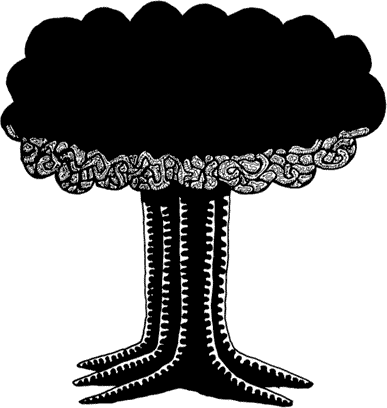
\includegraphics[height=2.5in]{Fig/GranMaPa} 			% automatically tries .png, .jpg, and .pdf

\bigskip
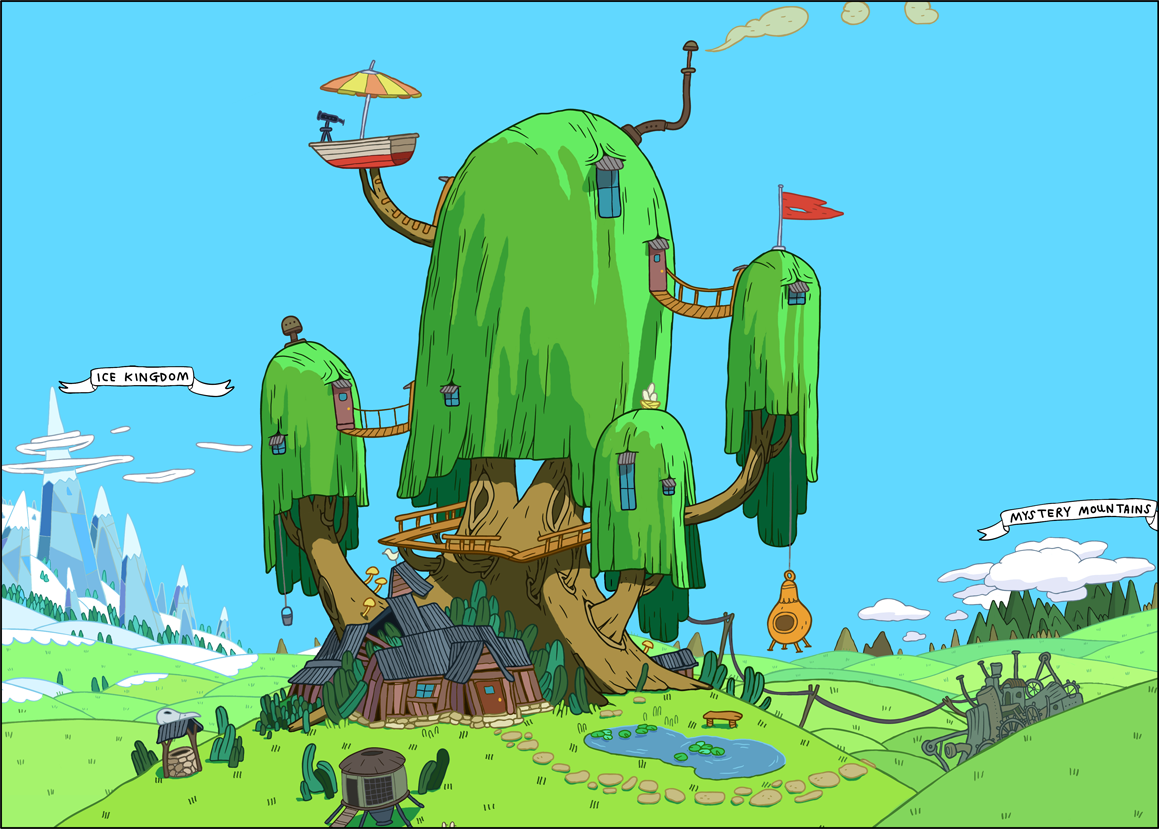
\includegraphics[height=2.5in]{Fig/FinnJakeTreehouse}
\end{center}
\end{solution}




\end{document}
